\par In order to achieve the ability to predict objects and scenes 
from FMRI images, a predictive model is required. The project was thus 
divided into a few main stages for independent preprocessing of the 
movie description and FMRI images, model building, and prediction
testing.

\begin{figure}[!htbp]
\centering
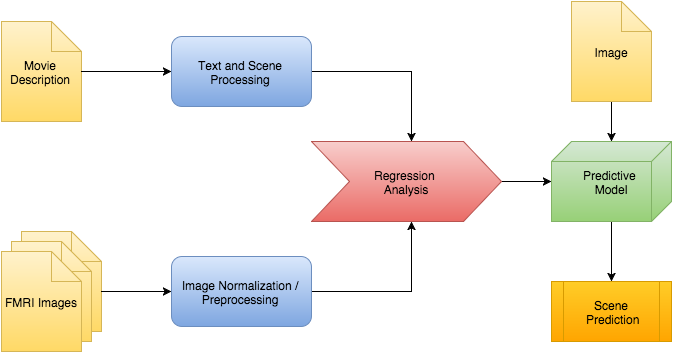
\includegraphics[width=0.6\textwidth]{processflow.png}
\caption{\label{fig:processflow} process flow of the project}
\end{figure}

\subsection{Text Preprocessing}
\subsubsection{Description Processing}
\par As the movie description was provided was in German, we first used Google
Translate to translate the description to English before proceeding with 
any further processing. Though there may be translational errors, it was decided that it was best to transform the original descriptions (versus using other English descriptions) to maintain the original time stamps from the researchers to have optimal alignment between the description and FMRI data.

\par Due to grammatical differences, we decided to only keep nouns and verbs, and discarded the adjectives and other words including stop-words, which are commonly used words with little meaning or determinable context (e.g. 'and', 'to', 'him'). A publicly available list of stop-words from Princeton University was used for this task, and iteratively appended to until our determined set of words contained no blatantly uninformative words. Of the words that remained, a WordNet dictionary was built, which is a popular way to tag words according to a context-specific definition, and classify them based on hierarchical similarities, eventually grouping English words into sets of synonyms called synsets. In this way, words as stand-alone entities will have an unambiguous definition and deeper relationships can be derived from the correlations found. 

 \par Word categories are determinable through WordNet, which classifies words based on hierarchical similarities and assigns semantic labels to distinguish between homophones, grouping English words into sets of synonyms called synsets.  
 \par After aggregating the set of all contextual definitions of words,
 we build a design matrix composed of the descriptive entries in the movie description. Thus each interval of time with a sentence description of the movie events was treated as a row, and each column represented a context-specific word as a feature. The matrix values are all binary, with a value of '1' indicating that the word is present at that time, while '0' indicates that it is not. This was illustrated as a rectangular image with a white square for '1' and black for '0'. 

\begin{figure}[!htbp]
\centering
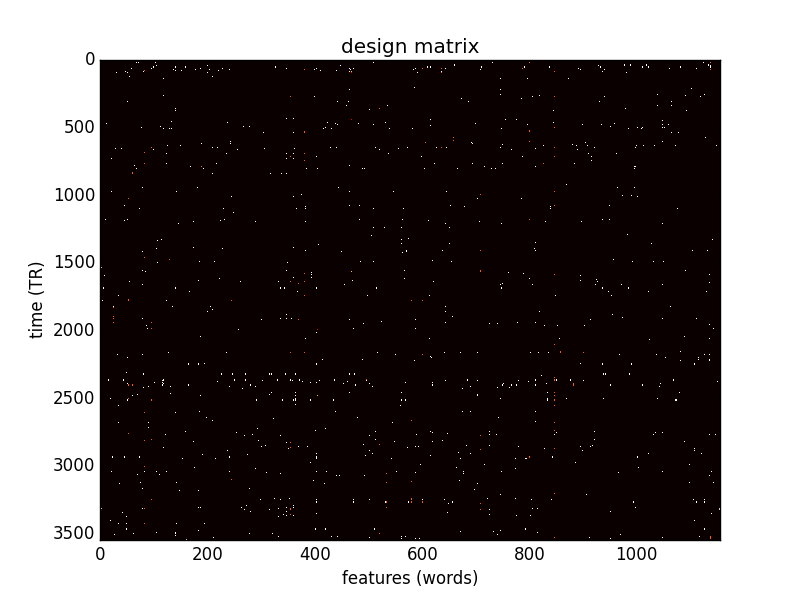
\includegraphics[width=0.5\textwidth]{design_matrix.png}
\caption{\label{fig:design_matrix} A visualization of design matrix for the semantic modeling}
\end{figure}

Finally, in order to format the data such that it correlates explicitly
to the FMRI images, the intervals were split into two-second intervals
to create a one-to-one representation between description objects and images. As can be seen in Figure 1 above, this matrix is quite sparse, as many words often appear for only a few seconds in the duration of the movie. 

\subsubsection{Scenes Processing}
\par The provided scenes file includes the start and end times of each of the 90 distinct movie scenes. We converted the scenes file into a csv (saved as 'scenes num times.csv' in the data folder) containing four columns: onset time, duration, amplitude, and factor id. The first time starts at 17 seconds because of credits, and most of the 90 distinct categories are very similar. For example, "Gump House" is in a separate category as "Gump Bedroom". Moreover, many scenes only occur once and only for a small fraction of time. Because of these similarities, we created the following scene categories: "Gump", "Military", "School", "Savanna", "Outside", and "Political". While these categories do not include every scene, they capture most of the scenes in the movie. For a more detailed list of the specific scenes that comprise each category, please look at 'scenes pred' script in the code folder.  

\subsection{FMRI Preprocessing}
\par The challenges underlying FMRI preprocessing include reforming the data to be properly representative of the subject, by correcting for inconsistencies in the data. \cite{lindquist2008statistical} Sources of these include temporal delays in scanning, spatial inconsistencies in subject location during imaging, and random noise from equipment and background during scanning. In the case of our fMRI data, spatial variability has been accounted for and corrected by the curators.

\subsubsection{Exploratory Analysis}
\par We first looked at different measures of spread such as IQR, standard deviation, and RMS for each voxel across time. The following plots (Figure 2 and Figure 3) below show the standard deviation and RMS differences of the voxel-time courses. Interesting to note is that the outliers seem to have, to some degree, structure in their location; the outliers seem to clump together in certain places. 
\par We also had to deal with the overlap of movie scenes. More specifically, during the beginning of a new segment/run, researchers replayed the last six seconds of the audiotape of the previous run. To deal with this, we dropped the last four volumes for runs two through seven. 

\begin{figure}[H]
\centering
\begin{minipage}{.5\textwidth}
  \centering
  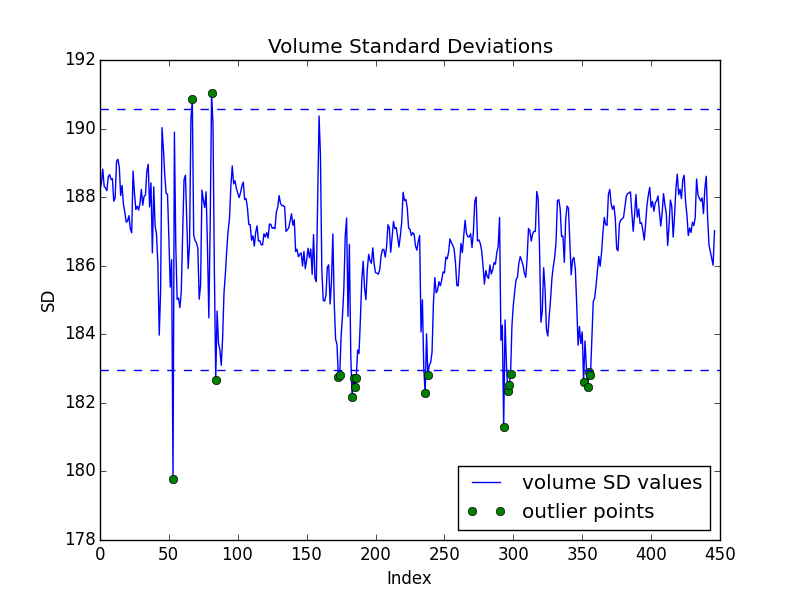
\includegraphics[width=.8\linewidth]{std_plt.png}
  \captionof{figure}{Standard deviation}
  \label{fig:test3}
\end{minipage}%
\begin{minipage}{.5\textwidth}
  \centering
  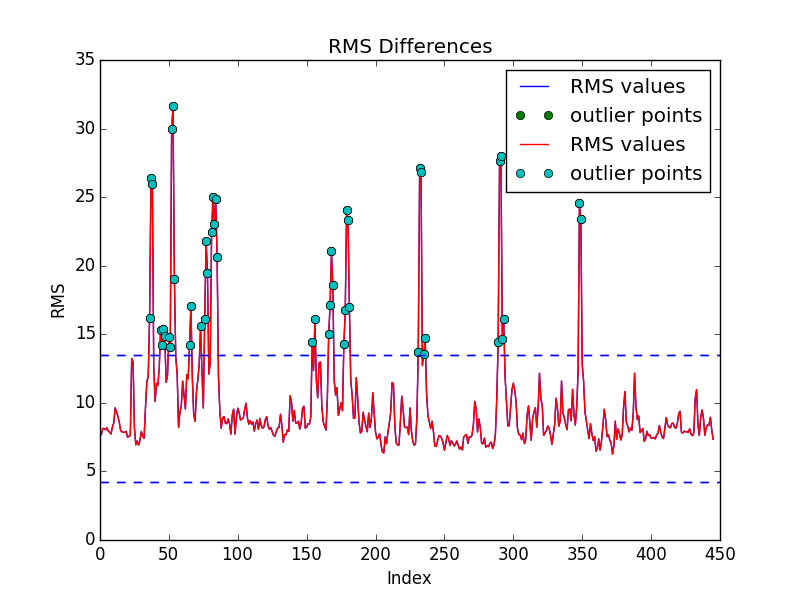
\includegraphics[width=.8\linewidth]{rms_outliers.png}
  \captionof{figure}{RMS(root mean squared differences)}
  \label{fig:test4}
\end{minipage}
\end{figure}


\subsubsection{Spatial Smoothing}
\par Our most preliminary step in preparing the data was to smooth each fMRI image by using a Gaussian Filter function from \texttt{SciPy}  (\texttt{ndimage.filters.gaussian\_filter}) to essentially blur the image slightly. This helps correct for noise which has been shown to be approximately random, voxel-independent, and centered around zero, thus permitting statistical requirements of the Gaussian filter. The Gaussian filter also maintains gradients in detected activity so spatial correlations are preserved, still allowing us to determine regions of brain activation for different concepts and words. This is significant for the purposes of increasing signal-to-noise ratio.
\par Multiple values of the Full Width at Half Maximum (FWHM) filter parameter were tested, with 3mm being selected as the ideal parameter for balance between adequately smoothing regions while maintaining definition of high-activity regions.

\begin{figure}[H]
\centering
\begin{minipage}{.5\textwidth}
  \centering
  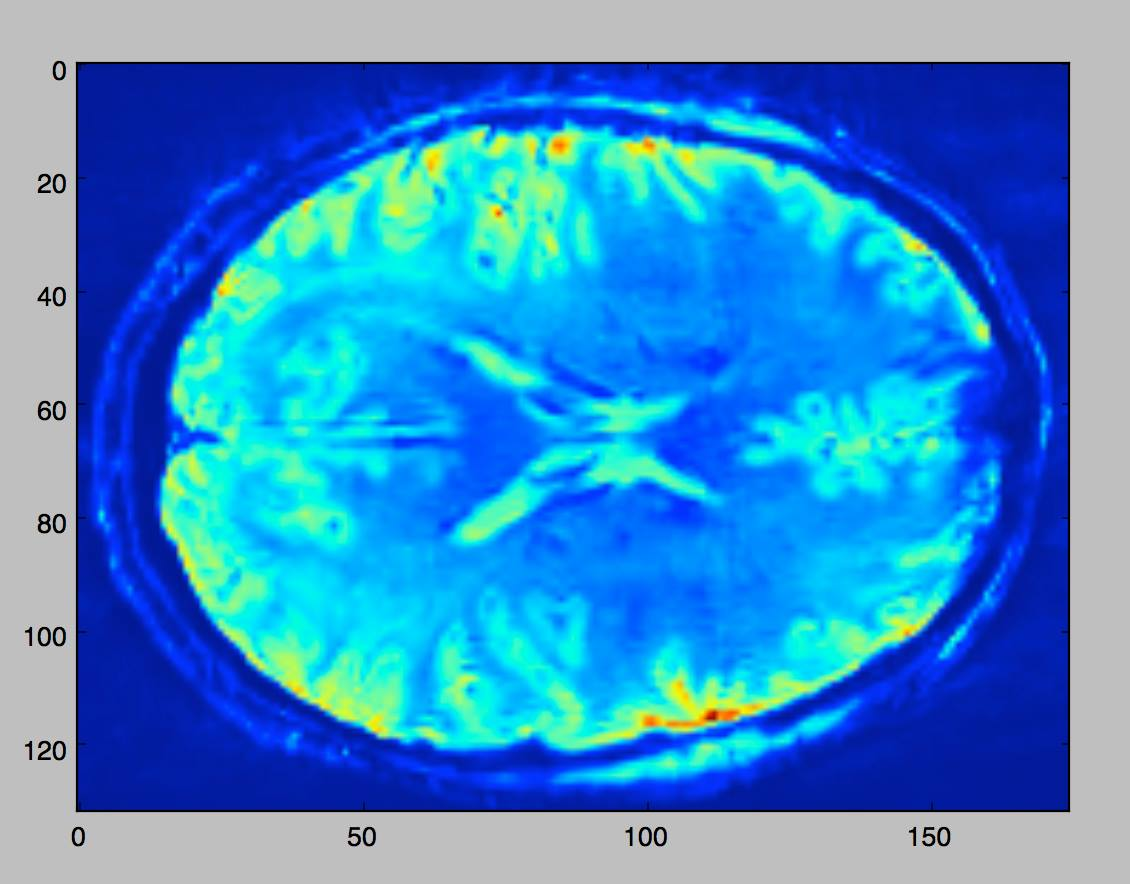
\includegraphics[width=.8\linewidth]{unsmoothed.jpg}
  \captionof{figure}{Raw fMRI image}
  \label{fig:test1}
\end{minipage}%
\begin{minipage}{.5\textwidth}
  \centering
  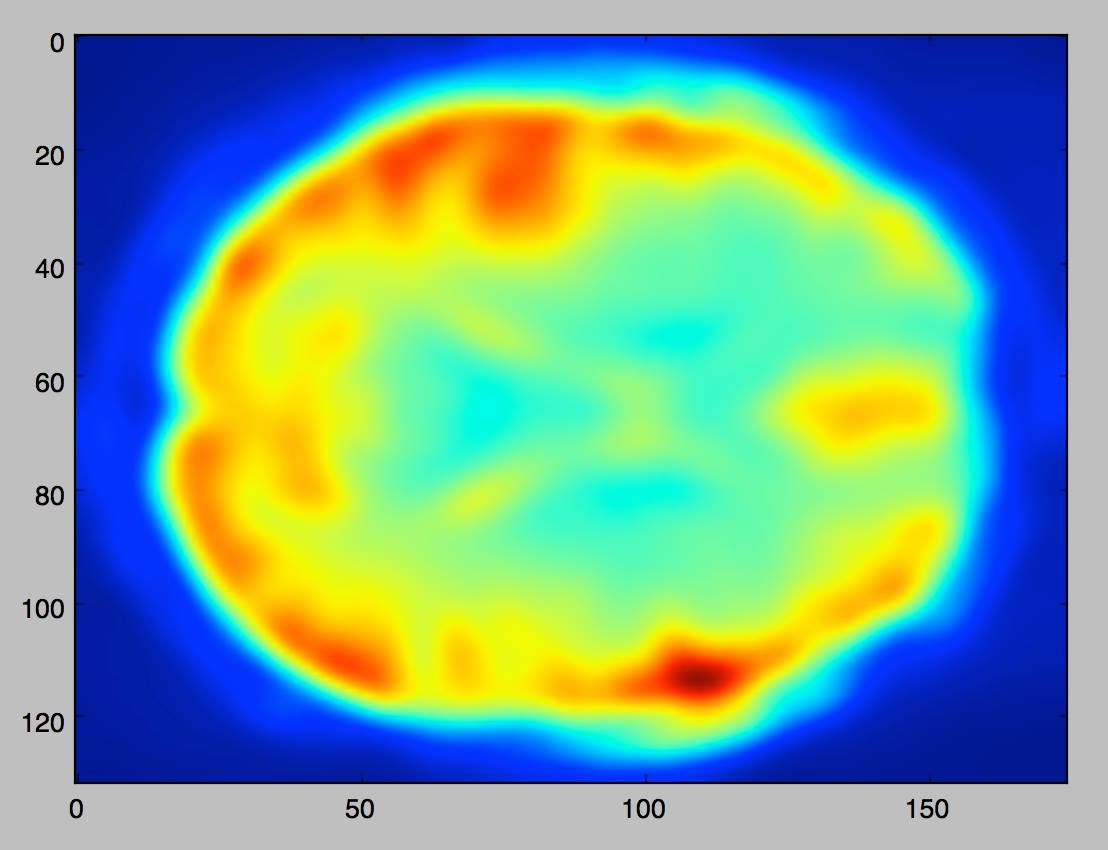
\includegraphics[width=.8\linewidth]{smoothed3mm.jpg}
  \captionof{figure}{Smoothed fMRI image, 3mm}
  \label{fig:test2}
\end{minipage}
\end{figure}

\par Figure 4 and Figure 5 represent a single fMRI image from our data. From a comparison between Figure 4 and Figure 5, notice that many of the sharp edges in the raw fMRI image have been blended with the surrounding areas. The minuscule red regions in the top and bottom areas of Figure 4 have been clearly increased, as well.  

\subsubsection{Temporal Filtering}
\par Given the smoothed images, the signal-to-noise ratio has been improved, equivalent to an amplification of the signal elements. At this point, we thus try to distinguish between the signal and noise and eliminate the noise elements. To this end, signal analyzers utilizing Fast-Fourier Transform (FFT) were used to identify low-frequency noise, and remove it. \texttt{Nitime}'s \texttt{analysis} package existed to help fulfill this task. 
\par The Fast-Fourier Transform	allows you to  
\par Again, as noise is voxel-wise independent, each voxel was analyzed and adjusted individually.

\begin{figure}[H]
\centering
\begin{minipage}{.5\textwidth}
	\centering
	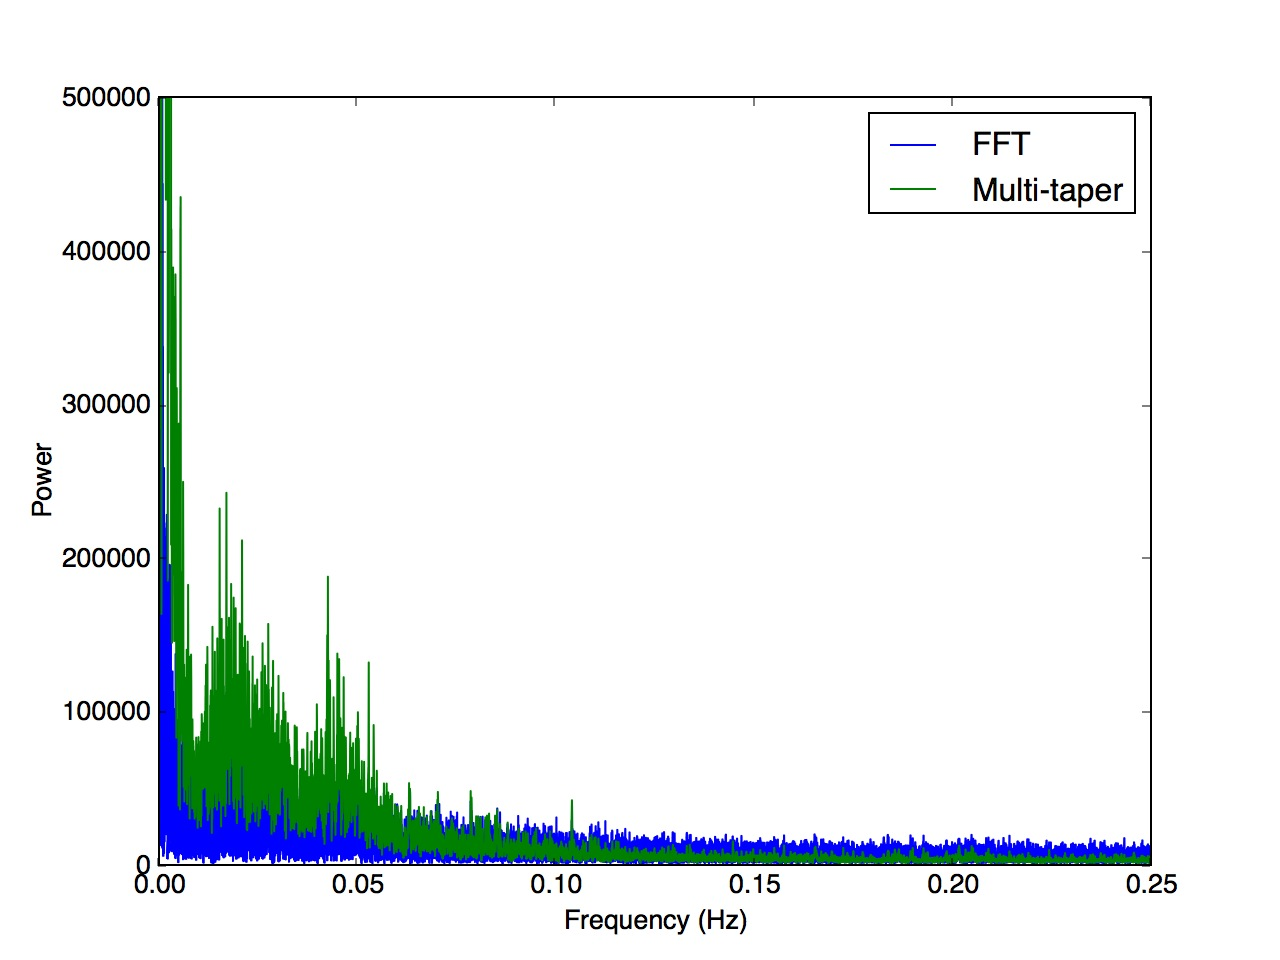
\includegraphics[width=.7\linewidth]{freq_decomp.jpg}
	\captionof{figure}{Voxel Frequency Decomposition}
	\label{fig:test5}
\end{minipage}%
\begin{minipage}{.5\textwidth}
  \centering
  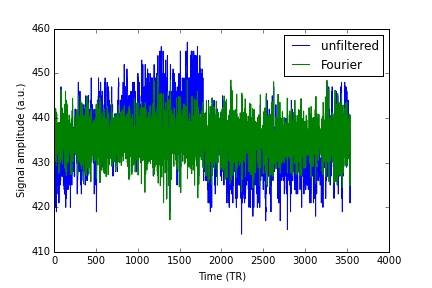
\includegraphics[width=.8\linewidth]{filtered_data.jpg}
  \captionof{figure}{Voxel Filtered Data}
  \label{fig:test1}
\end{minipage}
\end{figure}

\par Figure 6 illustrates the frequency decomposition for a voxel's signal, performed using \texttt{Nitime}'s \texttt{analysis.SpectralAnalyzer} module. There is a huge spike in low-frequency noise, manifesting in the unfiltered signal in Figure 7 as a wave along which the signal drifts. After filtering out this low-frequency noise using \texttt{nitime.analysis.FilterAnalyzer} (post-FFT), there is a noticeable increased in normality of the signal for a single voxel.

\subsubsection{Spatial Filtering}
\par Each of our fMRI scans at each time point occurred in dimensions of 132 x 175 x 48, for a total of 1,108,800  voxels per time point. With only approximately 3500 time points, our $m\times n$ data matrix becomes a case where $n >> m$ ($n$ voxels as features to describe a time point, $m$ number of timepoints). From a theoretical perspective, this is bad because excessive features promotes overfitting during any sort of analysis by giving repetitive and/or irrelevant features, and exponentially increasing the number of possible solutions (often referred to as \textit{The Curse of Dimensionality}). Practically, it also makes it difficult to perform analyses and machine learning for this volume of data due to hardware limitations. For these reasons, at this stage, we choose to reduce the number of voxels we consider in our analysis.
\par After taking care to amplify signal and remove noise, voxel values at this point reflect true values of BOLD activity. Voxels of interest are those that show significant variance in the subject. Since noisy waves/variation is removed, irrelevant voxels display approximately flat plots. 
\par We determine a boolean mask to apply to our data via taking the top $x$ voxels with highest variance. $x$ values considered were 50,000, 17,000, and 9,000 voxel subsets. These masks were visualized layered on the original image.

\begin{figure}[H]
\centering
\begin{minipage}{.5\textwidth}
  \centering
  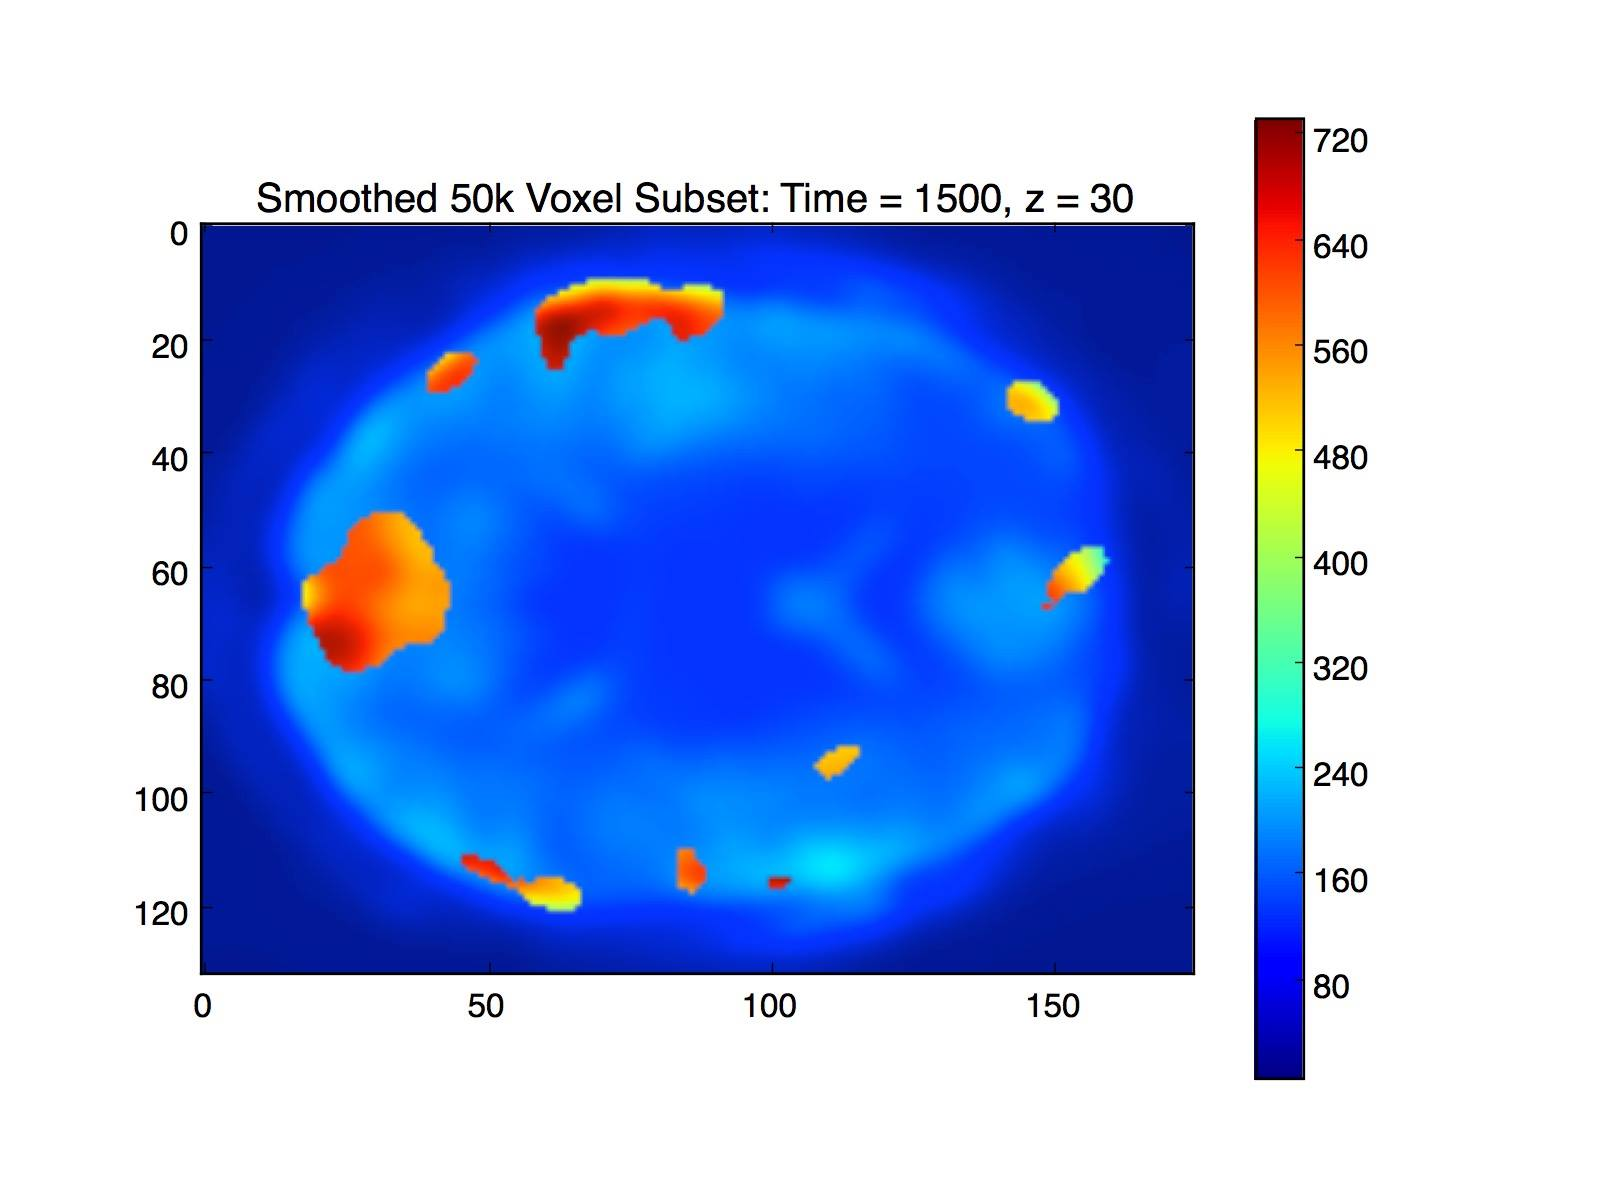
\includegraphics[width=.8\linewidth]{smooth50k.jpg}
  \captionof{figure}{50k mask}
  \label{fig:test1}
\end{minipage}%
\begin{minipage}{.5\textwidth}
  \centering
  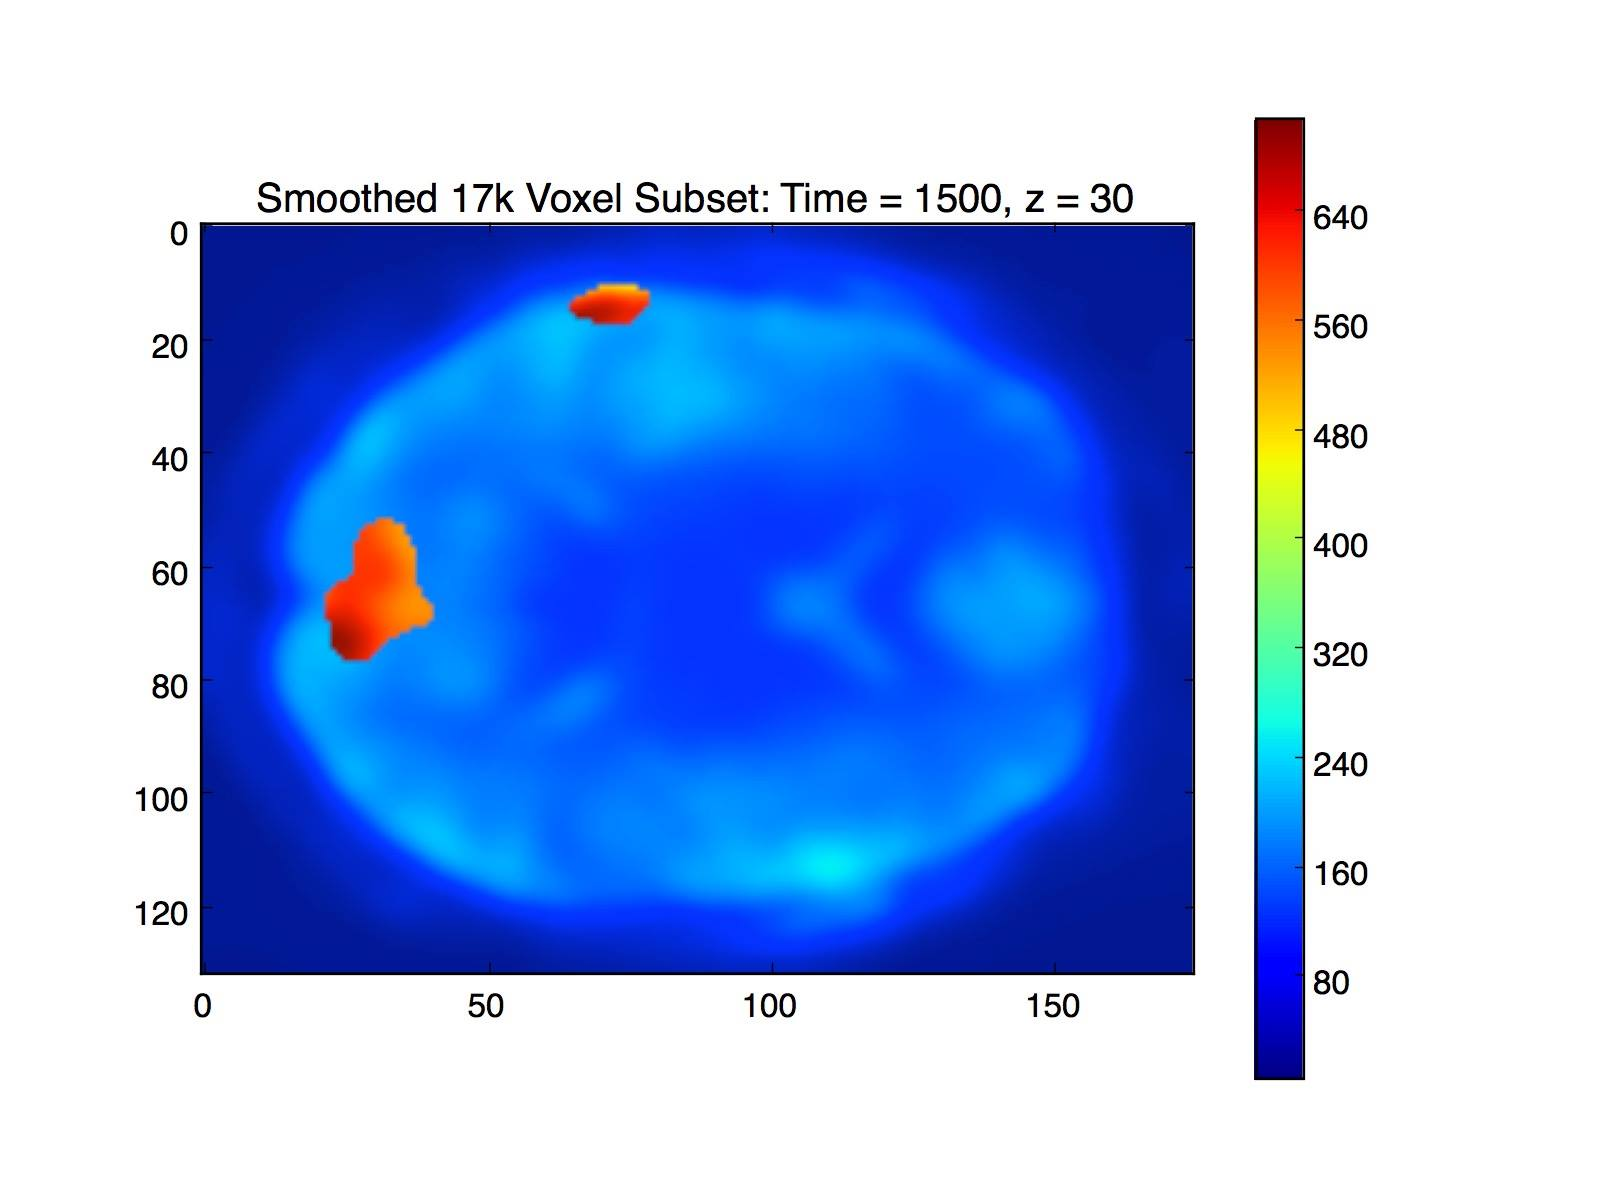
\includegraphics[width=.8\linewidth]{smooth17k.jpg}
  \captionof{figure}{17k mask}
  \label{fig:test2}
\end{minipage}
\begin{minipage}{.5\textwidth}
  \centering
  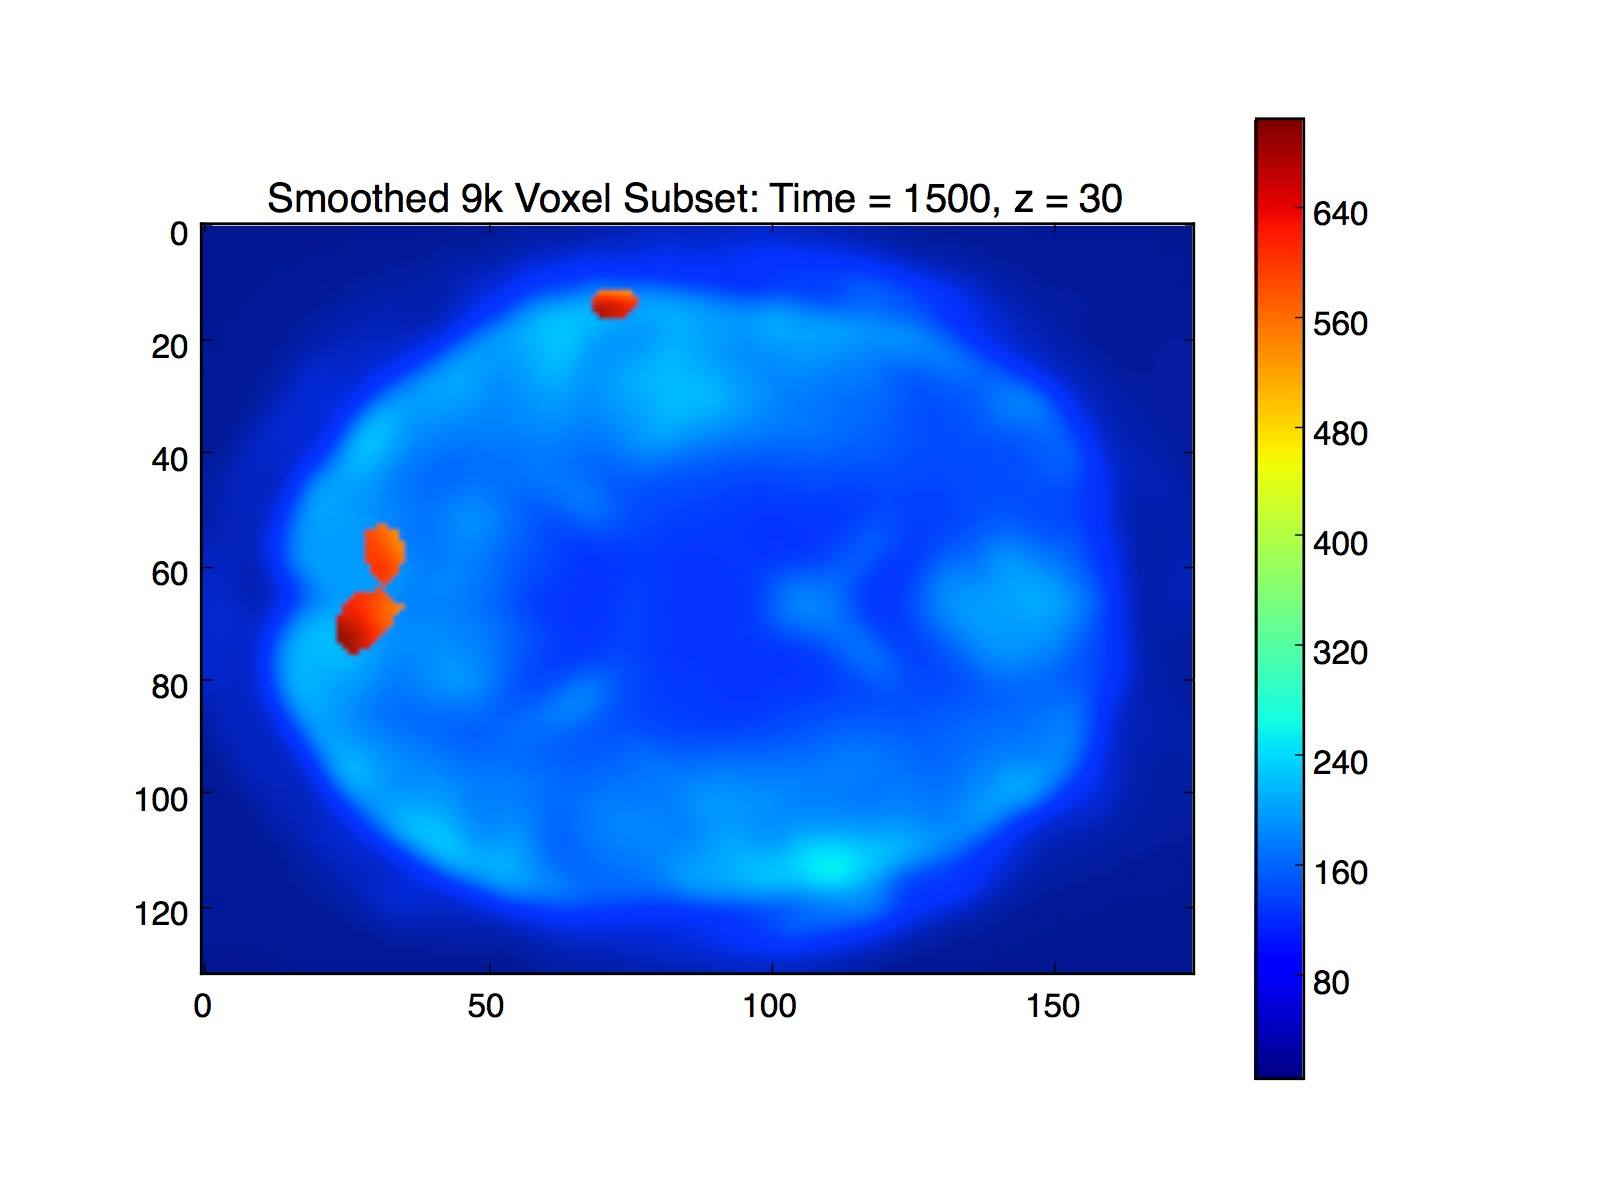
\includegraphics[width=.8\linewidth]{smooth9k.jpg}
  \captionof{figure}{9k mask}
  \label{fig:test2}
\end{minipage}
\end{figure}

\par As the 50k mask retained the most regional variability in brain regions covered, the 50k voxel mask was use in subsequent analyses, applied to the smoothed and filtered data.

\subsubsection{Normalization}
\par To ensure that the data is all scaled equally relative to each other, all of the data was normalized to have 0 mean and a standard deviation of 1, voxel-wise. For each $i$ voxels
$$ Z_i = \frac{X_i - \mu_i}{\sigma_i} $$  
The purpose of this was to ensure that features that span large ranges don't overshadow smaller but more significant features. By putting them on the same scale, this problem is averted.
\begin{figure}
  \centering
  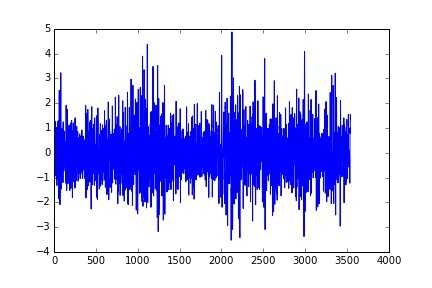
\includegraphics[width=.8\linewidth]{normalized_data.jpg}
  \captionof{figure}{Normalized Voxels}
  \label{fig:test1}
\end{figure}


\subsubsection{Time Lag Correction}
\par For ridge regression, three different time lags(2s,3s,4s) are added to the design matrix to model with the BOLD data.

\break

\subsection{Analysis and Modeling}
\subsubsection{K-Nearest Neighbors}
%please only write about method, there are another section for results
\par Though our end goal was to design a model for the data, we were interested to learn how strong the inherent structure of the data was. K-Nearest neighbors was therefore chosen as a method to test the predictive abilities of the data relative to each other.
\par The K-Nearest Neighbors is a supervised nonparametric predictive algorithm, requiring no training besides loading some data into the model. After that point, at test time, each data point is mapped into an $n$-dimensional hyperspace (where $n$ is the number of features describing it), and its predicted label is given as the majority label of the $k$ closest neighbors to it. If there exists a relationship between the voxel responses and scene categories, then there should exist some predictive power for scenes based on surrounding data points, 

\par In order to perform KNN clustering on our data (see \texttt{code/scenes pred.py} for specifics) we started off by creating a 'factor grid' that told us the ID of the scene the subject was listening to at each of the 3553 TRs. The next step was to pick out only a subset of the times that corresponded to scene categories of interest. For example, suppose we only had 5 TRs 1, 2, 3, 4, 5 and say the scenes that occurred during those times were A, C, B, A, C. Then if we we were only interested in scenes A and B, we would only choose  TRs 1, 3, and 4. Following this logic, we aggregated only the times at which a scene of interest occurred. For each scene we divided  90$\%$ of the times corresponding to that scene into training and testing samples. Let's call the fitting times $t = (t_1, t_2,..., t_n)$ and the corresponding factor id labels at these fitting times $l = (l_1, l_2, ..., l_n)$. Let $T = (T_1, T_2,..., T_k)$ and $L = (L_1, L_2, ..., L_k)$ be the times and labels for the testing sample. Using only 1500 voxels as our predictors (this subset was obtained using the filtering procedure specified in section 3.2), we created a subarray consisting of only the 1500 voxels and n fitting times. Call this n x 1500 matrix $m_{fit}$ and the k x 1500 testing matrix $M_{test}$. 
\par To execute the predictions this we used \texttt{Sklearn}'s \texttt{KNN} module to fit the design matrix $m_{fit}$ and known labels t. After fitting, we tested our model on $M_{test}$ and checked the proportion of the predicted labels that matched with T, the  true scene id labels.  

\subsubsection{Lasso and Ridge Regression}
\par Our goal with regression was to build an voxel-wise encoding model to predict voxel BOLD responses at a time, given the audio description for that time, similar to the paper aforementioned. The audio description design matrix was thus used with the voxel response value as the label, with a regression model built for each voxel. Thus for $n$ voxels ($n=55468$), we can construct $n$ $\beta$-weight matrices to predict each voxel value in $Y$
$$ \hat{Y} = f(X, \hat{B}), \hat{B} = [\hat{\beta}_1, \hat{\beta}_2, \ldots, \hat{\beta}_n ] $$

\par The design matrix we generated is relatively sparse, and thus penalty is imposed on the model weights. As shown in the semantic representation modeling paper\cite{stansbury2013neuron}, a L2 penalty on regression has a slightly better performance and easier implementation compared to L1 penalty. Thus we chose ridge regression as our first choice of regression techniques. The objective function of model for each voxel is:
$$\min_{w} \frac{1}{2n} ||Xw - y||_2^2 +\alpha||w||_2$$ 

We also look at $L_1$ Lasso Regression. The key difference between the two is that Lasso forces the coefficients of irrelevant features to be 0, functionally eliminating it, versus ridge regression simply reducing the values. This is due to the squaring in the $L_2$ regularization term, which tends to yield higher values than $L_1$'s simple sum. The attempted objective function to minimize is thus:
$$\min_{w} \frac{1}{2n} ||Xw - y||_2^2 +\alpha||w||_1$$ 

\par Ridge regression was implemented manually, modeled using 7/8 of the voxel activities as a training set and 1/8 of them as a testing set. The hyperparameter $\alpha$ is chosen with 10-fold cross-validation. Lasso regression was built using \texttt{sklearn}'s \texttt{linear\_model.Lasso} module, though a separate class interface was built similar to the scikit learn style in order to abstract away user interactions with the $B$ list of voxel regression models.
\subsubsection*{Accuracy Evaluation}
Following the paper\cite{stansbury2013neuron}, we computed the statistical significance threshold for the correlation $\rho$ at significance level $p<\alpha_{threshold}$. In the following, $t$ represents the critical value for a one-sided $t$-test, with the $(n-2)$ degree of freedom.
$$\rho_{threshold} = \frac{t}{\sqrt{t^2+n-2}} $$

\subsubsection{Neural Networks}
\par Though it deviates significantly from analysis attempts made by the paper we were following, we decided to build our own neural network as a decoding model, mostly out of curiosity. To simplify the objective for it, we restricted the problem statement to building a neural network that would predict the presence or absence of the most common words in the audio description. 

\par Neural networks are modeled loosely off of the human brain, containing layers of 'neurons' that take in inputs from all neurons in the previous layer ($X$), calculate some new value according to it's function weights ($z = XW$), and apply an activation function to adjust it before outputting to the next layer ($a = h(z)$). The 'learning' occurs in a supervised fashion, during a backpropagation step where the error of a predicted input is backpropagated to adjust the neuron weights. The network's goal is to minimize some cost function $J$ during training.

\begin{figure}[H]
  \centering
  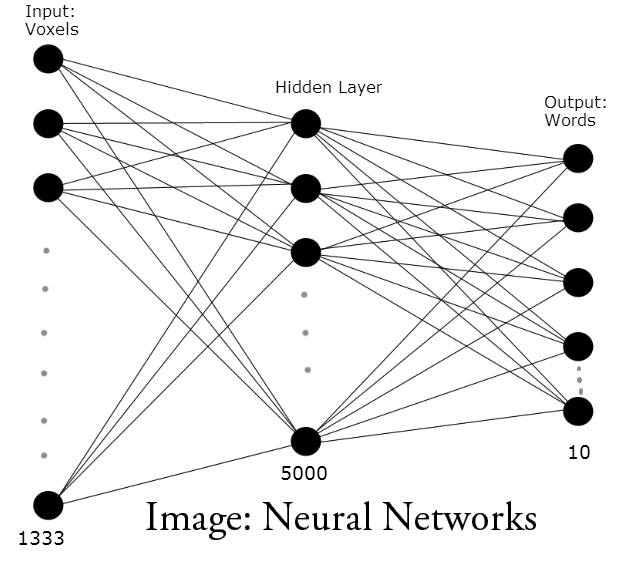
\includegraphics[width=.4\linewidth]{nn.jpg}
  \captionof{figure}{Neural Network Illustration}
  \label{fig:test1}
\end{figure}

\par Our network had an input layer, one 'hidden' intermediate layer, and an output layer. The size of the input layer was equal to the number of feature voxels, the hidden layer size was experimented with for multiple values but set at $n_{hidden} = 5000$, and for the ten words we aimed to predict for, $n_{out} = 10$. These choices were based on optimizations within the restrictions of our computational abilities. A Rectified Linear Unit (ReLU) activation function was used in the hidden layer ($h(z) = \max(0,z)$), and Sigmoid activator from the hidden layer to output layer ($h(z) = \frac{1}{1 + e^{-x}}$). The cost function used was the cost-entropy function, defined as
$$ J = -\sum_{k = 1}^{n_{out}} [y_k\ln h_k(x) + (1-y_k)\ln (1-h_k(x)] $$
We can thus determine the gradient of the cost to travel along as 
\begin{equation} \label{eq1}
\begin{split}
\frac{\partial J}{\partial w} & = \frac{\partial J}{\partial h} \frac{\partial h}{\partial w} \\
 & = -\sum_x \left(\frac{y}{h(x)} - \frac{1-y}{1-h(x)}\right) \frac{\partial h}{\partial w} \\
 & =-\sum_x \left(\frac{y}{h(x)} - \frac{1-y}{1-h(x)}\right) h'(x)
\end{split}
\end{equation}
In the case of ReLU, because it is not a smooth function, we approximate it using the softmax function $h(x) = \ln(1+e^x)$, whose derivative is simply the sigmoid function. For the derivative of the sigmoid function in the output layer, we have $\partial h(x) = h(x)(1-h(x))$. Using the gradient functions, the errors are backpropagated through the network to correct the weights.
\par The TanH function was also tried as an activation function for the input layer, which is a slightly steeper version of sigmoid. The derivative of the tanh function is $\partial h(x) = 1 - h(x)^2$. As the network trains, we also want to slowly decrease the weight of the error modifications, so we define a learning rate $\alpha$
$$ \alpha = \frac{4n}{10ia}$$
where $n$ is the total number of samples, $i$ is the current iteration, and $a$ is the accuracy at the time of learning rate modification (thus favoring lower changes high-accuracy weights). The learning rate was modified every epoch, defined as 100 iterations of stochastic gradient descent.

\begin{figure}
  \centering
  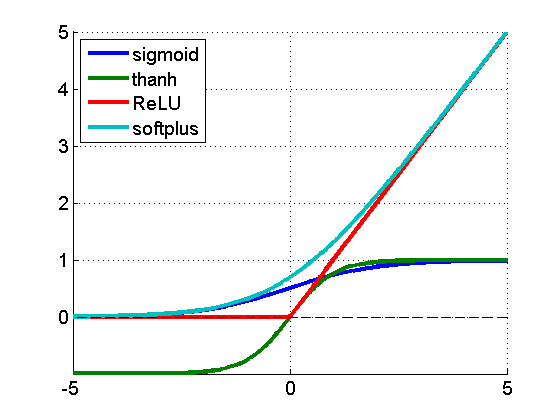
\includegraphics[width=.8\linewidth]{activation_funcs1.png}
  \captionof{figure}{Comparison of Activation Functions}
  \label{fig:test1}
\end{figure}

\par Due to the fully-connected property of layers, that each neuron in each layer inputs/outputs with every neuron in the layers before/after it, large layer sizes increase computational complexity very noticeably. Thus, though we had the 50,000 voxel subset, this was too many neurons for the input layer, and so it was reduced to approximately 5000. Training occurred on approximately 3200 time points, leaving approximately 300 for testing.










\break 
\break